\section{Search}

%\begin{comment}

  
\begin{frame}[fragile]{查找表}
  查找是许多应用系统中最消耗时间的一部分,一个好的查找算法会大大提高运行速度。计
  算机需要存储包含该特定信息的表,才可以高效查找。
\end{frame}


\begin{frame}[fragile]{查找表的分类}
  \begin{easylist} \easyitem
    & 静态查找表
    && 仅作查询和检索操作的查找表。
    & 动态查找表
    && 有时在查询之后,还需要将“查询”结果为“不在查找表中”的数据元素{\em 插入}到查找表中;或者,从查找表中{\em 删除}其“查询”结果为“在查找表中”的数据元素。
  \end{easylist}
\end{frame}


\begin{frame}[fragile]{关键字}
  \begin{easylist} \easyitem
    & 是数据元素(或记录)中某个数据项的值,用以标识(识别)一个数据元素(或记录)。
    & 若此关键字可以识别唯一的一个记录,则称之谓“主关键字”。
    & 若此关键字能识别若干记录,则称之谓“次关键字”。
    & 若数据元素只有一个数据项时,其关键字就是数据元素的值。
  \end{easylist}
\end{frame}


\begin{frame}[fragile]{查找}
  \begin{easylist} \easyitem
    & 根据给定的某个值,在查找表中确定一个其关键字等于给定值的数据元素或(记录)  
    & 若查找表中存在这样一个记录,则称“查找成功”:
    && 查找结果:给出整个记录的信息,或指示该记录在查找表中的位置;
    & 否则称“查找不成功”,查找结果:
    && 给出“空记录”或“空指针”。
    && 或者利用新的可选数据类型,例如Java中的Optional<Int>, Scala中的Option[Int]等
  \end{easylist}
\end{frame}


\begin{frame}[fragile]{如何进行查找?}
  \begin{easylist} \easyitem
    & 查找的方法取决于查找表的结构。
    & 如果查找表中的数据元素之间不存在明显的组织规律,就不利于快速查找
  \end{easylist}
\end{frame}


\begin{frame}[fragile]{本章大纲}
  \begin{center}
    \smartdiagram[bubble diagram]{查找表, 1. 静态查找表, 2. 动态查找表, 3. 哈希表}
  \end{center}
\end{frame}

\subsection{1. 静态查找表}
\begin{frame}[plain]
  \frametitle{}
  \centering
  \tikzstyle{mybox} = [draw=blue, fill=green!20, very thick,
  rectangle, rounded corners, inner sep=10pt, inner ysep=20pt]
  \tikzstyle{fancytitle} =[fill=blue, text=white, ellipse]
  
  \vspace{1.0cm}
  \begin{tikzpicture}[transform shape, rotate=0, baseline=-3.5cm]
    \node [mybox] (box) {%
      \begin{minipage}[t!]{0.75\textwidth}
        静态查找:对查找集合只进行查找,不涉及插入和删除操作。或者经过一段时间的查找之后,集中地进行插入和删除等修改操作。

        包括:

        \begin{itemize}
        \item 顺序查找
        \item 折半查找
        \item 分块查找
        \end{itemize}
      \end{minipage}
    };
    \node[fancytitle] at (box.north) {1. 静态查找表};
  \end{tikzpicture}
\end{frame}

\begin{frame}[fragile]
  \frametitle{顺序查找}
  \begin{easylist} \easyitem
    & 又称线性查找,是最基本的查找方法之一

    & 从表的一端向另一端逐个按给定值与关键码进行比较,若找到,查找成功,返回数据元素
    在表中的位置;若未找到与$k$相同的关键码,则返回失败信息。

    & 例:查找 $k=35$
  \end{easylist}
  
  \begin{center}
    \begin{tikzpicture}[box/.style={draw, inner sep=0.2cm, minimum size=1cm}]
      \draw[draw] node[box, fill=blue!20] (b0) {~}
      node[box, right=0 of b0] (b1) {10} 
      node[box, right=0 of b1] (b2) {15}
      node[box, right=0 of b2] (b3) {24}
      node[box, right=0 of b3] (b4) {6}
      node[box, right=0 of b4] (b5) {12}
      node[box, right=0 of b5, fill=red!10] (b6) {35}
      node[box, right=0 of b6] (b7) {40}
      node[box, right=0 of b7] (b8) {98}
      node[box, right=0 of b8] (b9) {55}; 

      \foreach \i in {0,...,9}
      {
        \draw node[above=0 of b\i] (idx_\i) {$\i$};
      };

      \path[] (b9.south) ++(0,-0.8cm) edge[-Latex, dashed] node[right]{$i$} (b9.south);
      \path[] (b6.south) ++(0,-0.8cm) edge[-Latex, very thick, draw=red] node[right]{$i$} (b6.south);

      \path[] (b8.south) ++(0,-1.2cm) edge[-Latex, very thick, draw=blue!60] node[above]{查找方向} ++(-6.5cm,0);
    \end{tikzpicture}
  \end{center}

  注意:下标为0的位置,其哨兵用途。
\end{frame}

\begin{frame}[plain]
  % Define box and box title style
  \tikzstyle{mybox} = [draw=red, fill=blue!20, very thick,
  rectangle, rounded corners, inner sep=10pt, inner ysep=20pt]
  \tikzstyle{fancytitle} =[fill=red, text=white]

  \begin{tikzpicture}
    \node [mybox] (box){%
      \begin{minipage}{0.80\textwidth}
        \begin{itemize}
        \item 分析查找算法的效率,通常用平均查找长度ASL (Average Search Length) 来衡
          量,即在查找成功时所进行的关键码比较次数的期望值。

          顺序查找(等概率情况下):

          \[
            ASL = \sum_{i=1}^{n}\dfrac{1}{n}(n-i+1) = \dfrac{n+1}{2}
          \]

          实际上,数据的查找概率存在相当大的差别!

        \item 在查找概率不同的情况下,应遵循查找表需依据查找概率越高,比较次数越少;查找概率
          越低,比较次数就较多的原则来存储数据元素。
        \end{itemize}
      \end{minipage}
    };
    \node[fancytitle, right=10pt] at (box.north west) {顺序查找的性能分析};
    % \node[fancytitle, rounded corners] at (box.east) {$\clubsuit$};
  \end{tikzpicture}
\end{frame}

\begin{frame}[fragile]
  \frametitle{顺序查找总结}
  \begin{easylist} \easyitem
    & 优点:算法简单而且使用面广。
    
    && 对表中记录的存储没有任何要求,顺序存储和链接存储均可(当然, 链式也只能用顺序
    查找);

    && 对表中记录的有序性也没有要求,无论记录是否按关键码有序均可。

    & 缺点:平均查找长度较大,特别是当待查找集合中元素较多时,查找效率较低。   
  \end{easylist}
\end{frame}

\begin{frame}[fragile]
  \frametitle{有序表的折半查找}
  \begin{easylist} \easyitem
    & 有序表是表中数据元素按关键码升序或降序排列。

    & 适用于:

    && 线性表中的记录必须按关键码有序;
    
    && 必须采用顺序存储。
  \end{easylist}
\end{frame}

\begin{frame}[fragile]
  \frametitle{请查找14}

  \scalebox{0.7}{
    \begin{tikzpicture}[box/.style={draw, inner sep=0.2cm, minimum size=1cm}]
      \draw[draw] node[box] (b0) {~}
      node[box, right=0 of b0] (b1) {7} 
      node[box, right=0 of b1] (b2) {14}
      node[box, right=0 of b2] (b3) {18}
      node[box, right=0 of b3] (b4) {21}
      node[box, right=0 of b4] (b5) {23}
      node[box, right=0 of b5] (b6) {29}
      node[box, right=0 of b6] (b7) {31}
      node[box, right=0 of b7] (b8) {35}
      node[box, right=0 of b8] (b9) {38}
      node[box, right=0 of b9] (b10) {42}
      node[box, right=0 of b10] (b11) {46}
      node[box, right=0 of b11] (b12) {49}
      node[box, right=0 of b12] (b13) {52} ; 

      \foreach \i in {0,...,13}
      {
        \draw node[above=0 of b\i] (idx_\i) {\i};
      };

      \path[] (b1.south) ++(0,-0.5cm) edge[-Latex, thick] node[below left]{$low=1$} (b1.south);
      \path[] (b13.south) ++(0,-0.5cm) edge[-Latex, thick] node[below right]{$high=13$} (b13.south);
      \path[] (b0.south) ++(-0.5cm,-1cm) edge[draw, dashed] node[above]{\textcircled{1} 设置初始区间} ++(14.5cm,0);


      \path[] (b7.south) ++(0,-1.6cm) edge[-Latex, thick] node[below]{$mid=7$} ++(0,0.5cm)  node[right, xshift=1cm]{\textcircled{2}调整到左半区};

      \path[] (b1.south) ++(0,-2.5cm) edge[-Latex, thick] node[below left]{$low=1$} ++(0,0.5cm);
      \path[] (b6.south) ++(0,-2.5cm) edge[-Latex, thick] node[below right]{$high=6$} ++(0,0.5cm);
      \path[] (b0.south) ++(-0.5cm,-3cm) edge[draw, dashed] node[above]{} ++(14.5cm,0);


      \path[] (b3.south) ++(0,-4cm) edge[-Latex, thick] node[below]{$mid=3$} ++(0,0.5cm)  node[right, xshift=1cm]{\textcircled{3}调整到左半区};

      \path[] (b1.south) ++(0,-4.8cm) edge[-Latex, thick] node[below left]{$low=1$} ++(0,0.5cm);
      \path[] (b2.south) ++(0,-4.8cm) edge[-Latex, thick] node[below right]{$high=2$} ++(0,0.5cm);
      \path[] (b0.south) ++(-0.5cm,-5.2cm) edge[draw, dashed] node[above]{} ++(14.5cm,0);


      \path[] (b1.south) ++(0,-6cm) edge[-Latex, thick] node[below]{$mid=1$} ++(0,0.5cm) node[right, xshift=1cm]{\textcircled{4}调整到右半区};

      \path[] (b2.south) ++(0,-6.8cm) edge[-Latex, thick] node[below left]{$low=2$} ++(0,0.5cm);
      \path[] (b2.south) ++(0,-6.8cm) edge[-Latex, thick] node[below right]{$high=2$} ++(0,0.5cm);
      \path[] (b0.south) ++(-0.5cm,-7.2cm) edge[draw, dashed] node[above]{} ++(14.5cm,0);

      
      \path[] (b2.south) ++(0,-8cm) edge[-Latex, thick] node[below]{$mid=2$} ++(0,0.5cm) node[right, xshift=1cm]{\textcircled{5}查找成功};
    \end{tikzpicture}
  } 
\end{frame}

\begin{frame}[fragile]
  \frametitle{课堂练习:请查找22}
  
  \scalebox{0.7}{
    \begin{tikzpicture}[box/.style={draw, inner sep=0.2cm, minimum size=1cm}]
      \draw[draw] node[box] (b0) {~}
      node[box, right=0 of b0] (b1) {7} 
      node[box, right=0 of b1] (b2) {14}
      node[box, right=0 of b2] (b3) {18}
      node[box, right=0 of b3] (b4) {21}
      node[box, right=0 of b4] (b5) {23}
      node[box, right=0 of b5] (b6) {29}
      node[box, right=0 of b6] (b7) {31}
      node[box, right=0 of b7] (b8) {35}
      node[box, right=0 of b8] (b9) {38}
      node[box, right=0 of b9] (b10) {42}
      node[box, right=0 of b10] (b11) {46}
      node[box, right=0 of b11] (b12) {49}
      node[box, right=0 of b12] (b13) {52} ; 

      \foreach \i in {0,...,13}
      {
        \draw node[above=0 of b\i] (idx_\i) {\i};
      };
    \end{tikzpicture}
  } 
\end{frame}

\begin{frame}[fragile]
  \frametitle{}
  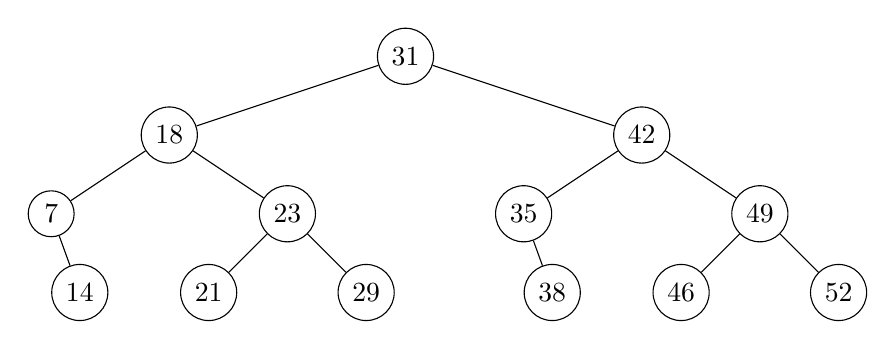
\begin{tikzpicture}[level distance=10mm]
    \tikzstyle{every node}=[draw,circle,inner sep=3pt, minimum size=0.5cm]
    \tikzstyle{level 1}=[sibling distance=60mm,
    set style={{every node}+=[]}]
    \tikzstyle{level 2}=[sibling distance=30mm,
    set style={{every node}+=[]}]
    \tikzstyle{level 3}=[sibling distance=20mm,
    set style={{every node}+=[]}]
    \node {31}
    child {node {18}
      child {node {7}         
        child[right] {node {14}}
      }
      child {node {23}
        child {node {21}}
        child {node {29}}
      }
    }
    child {node {42}
      child {node {35}
        child[right] {node {38}}
      }
      child {node {49}
        child {node {46}}
        child {node {52}}
      }
    };
  \end{tikzpicture}

  从折半查找过程看,以表的中点为比较对象,并以中点将表分割为两个子表,对定位到的子表
  继续这种操作。所以,对表中每个数据元素的查找过程,可用二叉树来描述。
  
  \begin{easylist} \easyitem
    & 折半查找在查找成功时,所进行的关键码比较次数至多为?
    
    & 请问平均查找长度(ASL)是多少?
  \end{easylist}
\end{frame}

\begin{frame}[fragile]
  \frametitle{}

  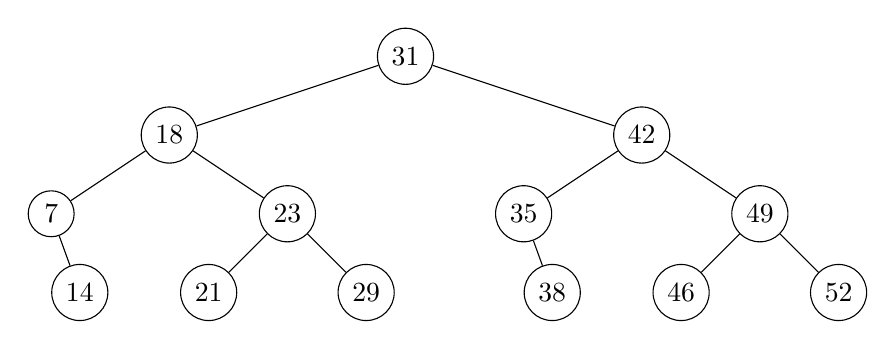
\begin{tikzpicture}[level distance=10mm]
    \tikzstyle{every node}=[draw,circle,inner sep=3pt, minimum size=0.5cm]
    \tikzstyle{level 1}=[sibling distance=60mm,
    set style={{every node}+=[]}]
    \tikzstyle{level 2}=[sibling distance=30mm,
    set style={{every node}+=[]}]
    \tikzstyle{level 3}=[sibling distance=20mm,
    set style={{every node}+=[]}]
    \node {31}
    child {node {18}
      child {node {7}         
        child[right] {node {14}}
      }
      child {node {23}
        child {node {21}}
        child {node {29}}
      }
    }
    child {node {42}
      child {node {35}
        child[right] {node {38}}
      }
      child {node {49}
        child {node {46}}
        child {node {52}}
      }
    };
  \end{tikzpicture}

  \begin{easylist} \easyitem
    & 折半查找在查找成功时,所进行的关键码比较次数至多为?

    \[
      \lfloor log_2 n \rfloor + 1
    \]
    
    & 请问平均查找长度(ASL)是多少?

    \[
      ASL = \dfrac{1}{n}[1 \times 2^0 + 2 \times 2^1 + \cdots + k \times  2^{k-1}]
      \approx \dfrac{n+1}{n} log_2(n+1) - 1
    \]   
  \end{easylist}
\end{frame}


\begin{frame}[fragile]
  \frametitle{分块查找/索引顺序查找}
  \begin{easylist} \easyitem

    & 分块查找又称索引顺序查找,是对顺序查找的一种改进。适用于表有序或者分块有
    序(后面的子表中所有记录的关键码均大于前一个子表的最大关键码)的情形。

    & 例:对某集合按关键码值31,62,88分为三块建立的查找表及其索引表如下:
  \end{easylist}
  
  \begin{center} 
  \scalebox{0.8}{
    \begin{tikzpicture}[box/.style={draw, minimum size=0.6cm},box2/.style={draw, minimum size=0.7cm, minimum width=1cm, fill=yellow!10}]
      \draw[draw] node[box] (b1) {14} 
      node[box, right=0 of b1] (b2) {31}
      node[box, right=0 of b2] (b3) {8}
      node[box, right=0 of b3] (b4) {22}
      node[box, right=0 of b4] (b5) {18}
      node[box, right=0 of b5] (b6) {43}
      node[box, right=0 of b6] (b7) {62}
      node[box, right=0 of b7] (b8) {49}
      node[box, right=0 of b8] (b9) {35}
      node[box, right=0 of b9] (b10) {52}
      node[box, right=0 of b10] (b11) {88}
      node[box, right=0 of b11] (b12) {78}
      node[box, right=0 of b12] (b13) {70} 
      node[box, right=0 of b13] (b14) {82}
      node[above left=0.2 of b1] {查找表}; 

      \foreach \i in {1,...,14}
      {
        \draw node[below=0 of b\i] (idx_\i) {\i};
      };

      \draw[draw] node[box2, above=1.5cm of b5] (x1) {31} 
      node[box2, right=0 of x1] (x2) {62}
      node[box2, right=0 of x2] (x3) {88}
      node[box2, below=0 of x1] (y1) {1}
      node[box2, below=0 of x2] (y2) {6}
      node[box2, below=0 of x3] (y3) {11}
      node[left=of x1] {索引表}
      node[right=0.2 of x3] {关键码字段}
      node[right=0.2 of y3] {指针字段};

      \path[draw] (y1.center) edge[-Latex] (b1.north) (y2.center) edge[-Latex] (b6.north) (y3.center) edge[-Latex] (b11.north);
    \end{tikzpicture}
  }
\end{center}
 
\end{frame}

\begin{frame}[fragile]
  \frametitle{分块查找}
  \begin{easylist} \easyitem

    & 分块查找要求将查找表分成若干个子表,并对子表建立索引表,查找表的每一个子表由
    索引表中的索引项确定。
    
    & 索引项

    && 关键码字段 (存放对应子表中的最大关键码值) ;
    && 指针字段 (存放指向对应子表的指针) ,并且要求索引项按关键码字段有序。
    
    & 如何根据索引表和查找表进行查找?
  \end{easylist}
  
  \begin{center} 
  \scalebox{0.8}{
    \begin{tikzpicture}[box/.style={draw, minimum size=0.6cm},box2/.style={draw, minimum size=0.7cm, minimum width=1cm, fill=yellow!10}]
      \draw[draw] node[box] (b1) {14} 
      node[box, right=0 of b1] (b2) {31}
      node[box, right=0 of b2] (b3) {8}
      node[box, right=0 of b3] (b4) {22}
      node[box, right=0 of b4] (b5) {18}
      node[box, right=0 of b5] (b6) {43}
      node[box, right=0 of b6] (b7) {62}
      node[box, right=0 of b7] (b8) {49}
      node[box, right=0 of b8] (b9) {35}
      node[box, right=0 of b9] (b10) {52}
      node[box, right=0 of b10] (b11) {88}
      node[box, right=0 of b11] (b12) {78}
      node[box, right=0 of b12] (b13) {70} 
      node[box, right=0 of b13] (b14) {82}
      node[above left=0.2 of b1] {查找表}; 

      \foreach \i in {1,...,14}
      {
        \draw node[below=0 of b\i] (idx_\i) {\i};
      };

      \draw[draw] node[box2, above=1.5cm of b5] (x1) {31} 
      node[box2, right=0 of x1] (x2) {62}
      node[box2, right=0 of x2] (x3) {88}
      node[box2, below=0 of x1] (y1) {1}
      node[box2, below=0 of x2] (y2) {6}
      node[box2, below=0 of x3] (y3) {11}
      node[left=of x1] {索引表}
      node[right=0.2 of x3] {关键码字段}
      node[right=0.2 of y3] {指针字段};

      \path[draw] (y1.center) edge[-Latex] (b1.north) (y2.center) edge[-Latex] (b6.north) (y3.center) edge[-Latex] (b11.north);
    \end{tikzpicture}
  }
\end{center}

\end{frame}

\begin{frame}[fragile]
  \frametitle{分块查找性能分析}

  \begin{easylist}
    & 分块查找含索引表查找和子表查找。
    
    & 设$n$个数据元素的查找表分为$b$个相同大小的块,每块含有$s$个记录,即:$b =
    \biggl \lceil \dfrac{n}{s}  \biggr \rceil $

    & 则分块查找的平均查找长度为:

    \[
      ASL=\dfrac{b+1}{2} + \dfrac{s+1}{2}
      = \dfrac{1}{2} \left (\dfrac{n}{s} + s \right )+1
    \]

    & 可见,平均查找长度和表的总长度$n$、每块的记录个数$s$有关。
  \end{easylist}
  \begin{center} 
  \scalebox{0.8}{
    \begin{tikzpicture}[box/.style={draw, minimum size=0.6cm},box2/.style={draw, minimum size=0.7cm, minimum width=1cm, fill=yellow!10}]
      \draw[draw] node[box] (b1) {14} 
      node[box, right=0 of b1] (b2) {31}
      node[box, right=0 of b2] (b3) {8}
      node[box, right=0 of b3] (b4) {22}
      node[box, right=0 of b4] (b5) {18}
      node[box, right=0 of b5] (b6) {43}
      node[box, right=0 of b6] (b7) {62}
      node[box, right=0 of b7] (b8) {49}
      node[box, right=0 of b8] (b9) {35}
      node[box, right=0 of b9] (b10) {52}
      node[box, right=0 of b10] (b11) {88}
      node[box, right=0 of b11] (b12) {78}
      node[box, right=0 of b12] (b13) {70} 
      node[box, right=0 of b13] (b14) {82}
      node[above left=0.2 of b1] {查找表}; 

      \foreach \i in {1,...,14}
      {
        \draw node[below=0 of b\i] (idx_\i) {\i};
      };

      \draw[draw] node[box2, above=1.5cm of b5] (x1) {31} 
      node[box2, right=0 of x1] (x2) {62}
      node[box2, right=0 of x2] (x3) {88}
      node[box2, below=0 of x1] (y1) {1}
      node[box2, below=0 of x2] (y2) {6}
      node[box2, below=0 of x3] (y3) {11}
      node[left=of x1] {索引表}
      node[right=0.2 of x3] {关键码字段}
      node[right=0.2 of y3] {指针字段};

      \path[draw] (y1.center) edge[-Latex] (b1.north) (y2.center) edge[-Latex] (b6.north) (y3.center) edge[-Latex] (b11.north);
    \end{tikzpicture}
  }
\end{center}

\end{frame}


\subsection{2. 动态查找表}
\begin{frame}[plain]
  \frametitle{}
  \centering
  \tikzstyle{mybox} = [draw=blue, fill=green!20, very thick,
  rectangle, rounded corners, inner sep=10pt, inner ysep=20pt]
  \tikzstyle{fancytitle} =[fill=blue, text=white, ellipse]
  
  \vspace{1.0cm}
  \begin{tikzpicture}[transform shape, rotate=0, baseline=-3.5cm]
    \node [mybox] (box) {%
      \begin{minipage}[t!]{0.75\textwidth}
        动态查找表的特点是,表结构本身是在查找过程中动态生成的,即对于给定的key,若
        表中存在其关键字等于key的记录,则查找成功返回,否则插入关键字等于key的记
        录。

        包括:

        \begin{itemize}
        \item 二叉排序树
        \item 平衡二叉树
        \end{itemize}
      \end{minipage}
    };
    \node[fancytitle] at (box.north) {2. 动态查找表};
  \end{tikzpicture}
\end{frame}

\begin{frame}[fragile]
  \frametitle{二叉排序树}
  \begin{columns}[T] % align columns
    \begin{column}{0.58\linewidth}
      \begin{itemize}
      \item 二叉排序树(Binary Sort Tree)或者是一棵空树;或者是具有下列性质的二叉树:

        \textcircled{1} 若左子树不空,则左子树上所有结点的值均小于根结点的值;若
        右子树不空,则右子树上所有结点的值均大于根结点的值。

        \textcircled{2} 左右子树也都是二叉排序树。

      \item 对二叉排序树进行中序遍历,可以得到一个按关键码有序的序列,因此,一个无序序列
        可通过构造二叉排序树而成为有序序列。
      \end{itemize}
    \end{column}
    \hfill
    \begin{column}{0.38\linewidth}
      \scalebox{0.7}{
        \begin{forest}
          [ 63
          [55
          [42  [10]    [45]  ]
          [58]
          ]
          [90
          [70 [67] [83]]
          [98]
          ]
          ]
        \end{forest}
      }
    \end{column}
  \end{columns}
\end{frame}

\begin{frame}[fragile]
  \frametitle{二叉排序树的查找}

  \begin{columns}[T] % align columns
    \begin{column}{0.58\linewidth}
      \begin{itemize}
      \item 若查找树为空,查找失败;否则将key与查找树的根结点比较

        \textcircled{1} 若相等,查找成功,否则,

        \textcircled{2} 如果key<根结点关键码,继续在以左子树上进行查找

        \textcircled{3} 如果key>根结点关键码,继续在以右子树上进行查找

      \item 例如在右图所示的树上查找45
      \end{itemize}
    \end{column}
    \hfill
    \begin{column}{0.38\linewidth}
      \scalebox{0.7}{
        \begin{forest}
          [ 63
          [55, edge={->, draw=red, thick}
          [42, edge={->, draw=red, thick}  [10]    [45, edge={->, draw=red, thick}]  ]
          [58]
          ]
          [90
          [70 [67] [83]]
          [98]
          ]
          ]
        \end{forest}
      }
    \end{column}
  \end{columns} 
\end{frame}

\begin{frame}[fragile]
  \frametitle{二叉排序树的查找(cont.)}

  \begin{minipage}{0.6\textwidth}
    \begin{easylist}
      & 两树的平均查找长度分别为:

      \[
        ASL_a = \dfrac{1}{6} \times [1+2+2+3+3+3] = \dfrac{14}{6}
      \]
      
      \[
        ASL_b = \dfrac{1}{6} \times [1+2+3+4+5+6] = \dfrac{21}{6}
      \]
      
      & 二叉排序树的平均查找长度和树的形态有关!最好情况是$O(log_2 n)$.
    \end{easylist}
  \end{minipage}%
  \begin{minipage}{0.36\textwidth}
    \scalebox{0.6}{
      \begin{forest}
        [45 [24 [12] [37]] [53,grow=-60 [93]]]
      \end{forest}
    }
    
    \scalebox{0.6} {
      \begin{forest}
        [12, grow=-45 [24, grow=-45 [37, grow=-45 [45, grow=-45 [53,grow=-60
        [93]]]]]]         
      \end{forest}
    }
  \end{minipage}
\end{frame}

\begin{frame}[fragile]
  \frametitle{二叉排序树的构建 --- 插入节点}
  \begin{minipage}{0.6\textwidth}
    \begin{itemize}
    \item 在查找不成功时,插入该key
      \begin{itemize}
      \item 新插入结点一定是作为叶子结点添加的
      \item 插入位置在查找过程中得到
      \end{itemize}
    \item 例如查找56
    \end{itemize}
  \end{minipage}%
  \begin{minipage}{0.36\textwidth}    
    \scalebox{0.6}{
      \begin{forest}
        [63 [55 [42 [10] [ 45]] [58, grow=245 [56, fill=red!50, dotted]]] [90 [70 [67] [83]] [98]]]
      \end{forest}
    }
  \end{minipage}
\end{frame}

\begin{frame}[fragile]
  \frametitle{序列: 63, 90, 70, 55, 67, 42, 98, 83, 10, 45, 58}
  \small
  \scalebox{0.65}{
    \begin{forest}
      [63]
    \end{forest}\quad
    \begin{forest}
      [63 [, missed] [90, fill=red!10]]
    \end{forest}\quad
    \begin{forest}
      [63 [, missed] [90 [70, fill=red!10] [, missed]]]
    \end{forest}\quad
    \begin{forest}
      [63 [55, fill=red!10] [90 [70] [, missed]]]
    \end{forest}\quad
    \begin{forest}
      [63 [55] [90 [70 [67,fill=red!10] [, missed]] [, missed]]]
    \end{forest}\quad
    \begin{forest}
      [63 [55 [42,fill=red!10] [, missed]] [90 [70 [67] [, missed]] [, missed]]]
    \end{forest}\quad
    \begin{forest} 
      [63 [55 [42] [, missed]] [90 [70 [67] [, missed]] [98, fill=red!10]]]
    \end{forest}
  }

  \scalebox{0.6}{
    
    \begin{forest} 
      [63 [55 [42] [, missed]] [90 [70 [67] [83, fill=red!10]] [98]]]
    \end{forest}
    \quad
    \begin{forest} 
      [63 [55 [42 [10, fill=red!10] [,missed]] [, missed]] [90 [70 [67] [83]] [98]]]
    \end{forest}
    \quad
    \begin{forest} 
      [63 [55 [42 [10] [45, fill=red!10]] [, missed]] [90 [70 [67] [83]] [98]]]
    \end{forest}
    \quad
    \begin{forest} 
      [63 [55 [42 [10] [45]] [58, fill=red!10]] [90 [70 [67] [83]] [98]]]
    \end{forest}
  }
\end{frame}

\begin{frame}[fragile]
  \frametitle{二叉排序树的删除操作}

  依次删除结点45、90,仍要使树保持二叉排序树的特性

  \begin{columns}[T]
    \column{0.4\textwidth}
    \begin{forest} 
      [63 [55 [42 [,missed] [45, fill=red!20]] [58]] [90, fill=blue!20 [70 [67] [83]] [, missed]]]
    \end{forest}

    \column{0.6\textwidth}
    \begin{itemize}
    \item 待删结点p为叶结点

      ~~ 直接删除即可(如节点45)
    \item 待删结点p只有右子树或只有左子树

      ~~ 用子树的根代替之(如节点90)
    \item 待删结点p有右子树也有左子树?

      ~~ 原则:保持中序遍历序列不变!
    \end{itemize}
  \end{columns}
\end{frame}

\begin{frame}[fragile]
  \frametitle{二叉排序树的删除操作}

  删除节点55:
  
  \begin{columns}[T]
    \column{0.4\textwidth}
    \begin{forest} 
      [63 [55, fill=red!20 [42 [,missed] [45]] [58]] [90 [70 [67] [83]] [, missed]]]
    \end{forest}

    \column{0.6\textwidth}
    方法1: 用前驱代替

    \begin{forest} 
      [63 [45, fill=blue!20 [42] [58]] [90 [70 [67] [83]] [, missed]]]
    \end{forest}
  \end{columns}
\end{frame}

\begin{frame}[fragile]
  \frametitle{二叉排序树的删除操作}

  删除节点55:
  
  \begin{columns}[T]
    \column{0.4\textwidth}
    \begin{forest} 
      [63 [55, fill=red!20 [42 [,missed] [45]] [58]] [90 [70 [67] [83]] [, missed]]]
    \end{forest}

    \column{0.6\textwidth}
    方法2: 用后继代替

    \begin{forest} 
      [63 [58, fill=green!20 [42, [, missed] [45]] [,missed]] [90 [70 [67] [83]] [, missed]]]
    \end{forest}
  \end{columns}
\end{frame}

\begin{frame}[fragile]
  \frametitle{二叉排序树的删除操作}

  删除节点55:
  
  \begin{columns}[T]
    \column{0.4\textwidth}
    \begin{forest} 
      [63 [55, fill=red!20 [42 [,missed] [45]] [58, fill=green!20]] [90 [70 [67] [83]] [, missed]]]
    \end{forest}

    \column{0.6\textwidth}

    方法3: 用左子树的根代替之,并将右子树作为删除结点的前驱的右子树

    \begin{forest} 
      [63 [42, fill=red!10 [,missed] [45, [, missed] [58, fill=green!20]]] [90 [70 [67] [83]] [, missed]]]
    \end{forest}
  \end{columns}
\end{frame}

\begin{frame}[fragile]
  \frametitle{课堂练习}

  给定关键字序列:63, 90, 70, 55, 67, 42, 98, 83, 10, 45, 58

  \begin{itemize}
  \item 构建二叉排序树
  \item 对该树中序遍历,显示其序列
  \item 依次删除10,42,63
  \item 再次对该树中序遍历,显示其序列
  \end{itemize}
\end{frame}

\subsubsection{平衡二叉树}
\begin{frame}[fragile]
  \frametitle{平衡二叉树}

  在二叉查找树中,若输入元素的顺序接近有序,那么二叉查找树将退化为链表,从而导致二叉
  查找树的查找效率大为降低。如何使得二叉查找树无论在什么样情况下都能使它的形态最
  大限度地接近满二叉树以保证它的查找效率呢?

  前苏联科学家G.M. Adelson-Velskii 和 E.M. Landis在1962年发表的一篇名为An
  algorithm for the organization of information的文章中提出了一种自平衡二叉查找
  树(self-balancing binary search tree)。

  该树在插入和删除操作中,通过一系列的旋转操作来保持平衡,从而保证了二叉查找树的查
  找效率。最终这种二叉查找树以他们的名字命名为“AVL-Tree”。  
\end{frame}

\begin{frame}[fragile]
  \frametitle{平衡二叉树(AVL)}
  
  平衡二叉树(Balanced binary tree)或者是一棵空树,或者是具有下列性质的二叉排序树:

  \begin{itemize}
  \item 它的左子树和右子树都是平衡二叉树,且左子树和右子树高度之差的绝对值不超过1。
  \item 平衡因子=左子树高度-右子树高度
  \end{itemize}

  
  \begin{columns}[T]
    \column{0.5\textwidth}
    \hspace{1cm}
    \scalebox{0.5}{
      \begin{tikzpicture}[n/.style={draw, minimum size=1cm, circle}]
        \draw node[n] (n1) {90}  node[right=0 of n1] {\color{red} -1}
        node[n, below left=of n1, xshift=5](n2){83}  node[right=0 of n2] {\color{red} 0}
        node[n, below right=of n1, xshift=-5](n3){95}  node[right=0 of n3] {\color{red} -1}
        node[n, below right=of n3, xshift=-5](n4){98} node[right=0 of n4] {\color{red} 0};

        \path[draw] (n1) -- (n2);
        \path[draw] (n1) -- (n3) --(n4);
      \end{tikzpicture}
    }
    
    \column{0.5\textwidth}
    \scalebox{0.5}{
      \begin{tikzpicture}[n/.style={draw, minimum size=1cm, circle}]
        \draw node[n] (n1) {9} 
        node[n, below=of n1, xshift=-1cm](l2){7} 
        node[n, below=of l2, xshift=-1cm](l3){5} 
        node[n, below=of l3, xshift=-1cm](l4){3}
        node[n, below=of n1, xshift=1cm](r2){10} 
        node[n, below=of r2, xshift=1cm](r3){12} 
        node[n, below=of r3, xshift=1cm](r4){14};

        \path[draw] (n1) -- (l2) --(l3) --(l4);
        \path[draw] (n1) -- (r2) --(r3) --(r4);
      \end{tikzpicture}
    }
  \end{columns}

\end{frame}

\begin{frame}[fragile]
  \frametitle{二叉子树的平衡化}
  \begin{itemize}
  \item 在平衡二叉树上插入新结点,可能会导致不平衡!
  \item 请问哪些结点的平衡因子发生变化?
  \end{itemize}

  \includegraphics[width=1.0\textwidth]{figs/AVL-1.png}
\end{frame}

\begin{frame}[fragile]
  \frametitle{二叉子树的平衡化(cont.)}
  平衡化调整的原则:
  \begin{itemize}
  \item 转换后的二叉树的中序遍历不变;
  \item 每次转换都要平衡。
  \end{itemize}

  四种情形:

  \begin{center}
    \begin{tabular}{c c c c}
      单向右旋 & 先左后右双向旋转 & 单项左旋 & 先右后左双向旋转 \\
      \scalebox{0.5}{
      \begin{forest}
        for tree={fill=white, color=white, draw=black, minimum size=1cm}
        [1 [2 [4 [6] [,missed]] [5]] [3]]
      \end{forest}
      }
               &
      \scalebox{0.5}{
       \begin{forest}
         for tree={fill=white, color=white, draw=black, minimum size=1cm}
	       [1 [2 [4] [5 [,missed] [6]]] [3]]
       \end{forest}
      }
                                  &
      \scalebox{0.5}{
      \begin{forest}
        for tree={fill=white, color=white, draw=black, minimum size=1cm}
        [1 [2] [3 [4] [5 [,missed] [6]]]]
      \end{forest}
      }                                    
                                             &
      \scalebox{0.5}{
      \begin{forest}
        for tree={fill=white, color=white, draw=black, minimum size=1cm}
        [1 [2] [3 [4 [6] [,missed]] [5]]]
      \end{forest}
      }                                               
    \end{tabular}
  \end{center}
\end{frame}

\begin{frame}[fragile]
  \frametitle{单向右旋}
  \includegraphics[width=0.8\textwidth]{figs/AVL-4.png}
\end{frame}


\begin{frame}[fragile]
  \frametitle{单向左旋}
  \includegraphics[width=0.8\textwidth]{figs/AVL-5.png}
\end{frame}


\begin{frame}[fragile]
  \frametitle{先左后右双向旋转}
  \includegraphics[width=0.8\textwidth]{figs/AVL-6.png}
\end{frame}


\begin{frame}[fragile]
  \frametitle{先右后左双向旋转}
  \includegraphics[width=0.8\textwidth]{figs/AVL-7.png}
\end{frame}


\begin{frame}[fragile]
  \frametitle{Why double rotation?}
  \includegraphics[width=0.8\textwidth]{figs/AVL-8.png}
\end{frame}

\begin{frame}[fragile]
  \frametitle{练习}
  \begin{itemize}
  \item 输入关键字序列16,3,7,11,9,26,18,14,15
  \item 构造一个AVL树
  \end{itemize}

  AVL tree visualization:
  \url{https://www.cs.usfca.edu/\~galles/visualization/AVLtree.html}
\end{frame}

\begin{frame}[fragile]
  \frametitle{序列:16,3,7,11,9,26,18,14,15}

  \scalebox{0.5}{
    \begin{forest}
      for tree={minimum size=1cm}
      [16 [3 [, missed] [7]] [, missed]]
    \end{forest}

    \begin{forest}
      for tree={minimum size=1cm}
      [16 [7 [3] [, missed]] [, missed]]
    \end{forest}

    \begin{forest}
      for tree={minimum size=1cm}
      [7 [3] [16]]
    \end{forest}

    \begin{forest}
      for tree={minimum size=1cm}
      [7 [3] [16 [11] [, missed]]]
    \end{forest}
    
    \begin{forest}
      for tree={minimum size=1cm}
      [7 [3] [16 [11 [9] [,missed]] [, missed]]]
    \end{forest}

    \begin{forest}
      for tree={minimum size=1cm}
      [7 [3] [11 [9] [16]]]
    \end{forest}
    
    \begin{forest}
      for tree={minimum size=1cm}
      [7 [3] [11 [9] [16 [,missed] [26]]]]
    \end{forest}
  }

  \scalebox{0.5}{
    \begin{forest}
      for tree={minimum size=1cm}
      [11 [7 [3] [9]] [16 [,missed] [26]]]
    \end{forest}

    \begin{forest}
      for tree={minimum size=1cm}
      [11 [7 [3] [9]] [16 [,missed] [26 [18] [,missed]]]]
    \end{forest}

    \begin{forest}
      for tree={minimum size=1cm}
      [11 [7 [3] [9]] [18 [16] [26]]]
    \end{forest}

    \begin{forest}
      for tree={minimum size=1cm}
      [11 [7 [3] [9]] [18 [16 [14] [,missed]] [26]]]
    \end{forest}
  }
\end{frame}

\begin{frame}[fragile]
  \frametitle{序列:16,3,7,11,9,26,18,14,15}
  \scalebox{0.5}{
    \begin{forest}
      for tree={minimum size=1cm}
      [11 [7 [3] [9]] [18 [16 [14 [,missed] [15]] [,missed]] [26]]]
    \end{forest}

    \begin{forest}
      for tree={minimum size=1cm}
      [11 [7 [3] [9]] [18 [16 [15 [14] [,missed]] [,missed]] [26]]]
    \end{forest}
    
    \begin{forest}
      for tree={fill=red!10, minimum size=1cm}
      [11 [7 [3] [9]] [18 [15 [14] [16]] [26]]]
    \end{forest}    
  }
\end{frame}


%\end{comment}

\subsection{3. 哈希表}

\begin{frame}[plain]
  \frametitle{}
  \centering
  \tikzstyle{mybox} = [draw=blue, fill=green!20, very thick,
  rectangle, rounded corners, inner sep=10pt, inner ysep=20pt]
  \tikzstyle{fancytitle} =[fill=blue, text=white, ellipse]
  
  \vspace{1.0cm}
  \begin{tikzpicture}[transform shape, rotate=0, baseline=-3.5cm]
    \node [mybox] (box) {%
      \begin{minipage}[t!]{0.75\textwidth}
        哈希是一种重要的存储方法,也是一种重要的查找方法。其基本思想是以关键字为
        自变量,使用哈希函数映射到地址集合,那么根据哈希函数便可以直接找到包含该
        关键字的集合的存储地址。
      \end{minipage}
    };
    \node[fancytitle] at (box.north) {3. 哈希表};
  \end{tikzpicture}
\end{frame}

\begin{frame}[fragile]
  \frametitle{Think}
  \begin{itemize}
  \item 顺序查找
  \item 折半查找
  \item 分块查找
  \item 二叉查找树
  \end{itemize}
  
  对给定值和关键字进行比较,查找效率由比较一次缩小的查找范围决定。

  能否直接定位到给定值的存储位置,不用逐步缩小查找范围?
\end{frame}

\begin{frame}[fragile]
  \frametitle{哈希表}
  \begin{itemize}
  \item 哈希方法:选取某个函数,依据关键字直接得到其对应的数据元素的存储位置。也
    有的将哈希译为散列。
  \item 哈希方法中使用的转换函数称为哈希函数。按这个思想构造的表称为哈希表。
  \end{itemize}
\end{frame}

\begin{frame}[fragile]
  \frametitle{Example}
  \begin{tabular}{| c | c | c | }
    \hline
    Name & Cellphone & Affiliate \\ \hline
    Zhang & 138{\color{red}0001}1234 & RUC \\ \hline
    Wang & 138{\color{red}0002}1235 & RUC \\ \hline
    Zhao & 138{\color{red}0003}8322 & IRM \\ \hline
    Qian & 138{\color{red}0004}7322 & IRM \\ \hline
  \end{tabular}

  \begin{itemize}
  \item 该例子中我们可以直接利用红色部分作为存储单元的位置。
  \item 理想的哈希函数应该运算简单并保证不同的关键字映射到不同单元,但这是不可能
    的。冲突不可避免,只能尽量减少。
  \item 存储单元涉及的范围不要过大
  \end{itemize}

  哈希方法需要解决的两个问题:
  \begin{itemize}
  \item 构造好的哈希函数
  \item 制定解决冲突的方案
  \end{itemize}
\end{frame}

\begin{frame}[fragile]
  \frametitle{Hash函数的构造方法}
  \begin{itemize}
  \item Hash地址(函数值) 分布应均匀

    函数值尽量均匀散布在地址空间,保证空间有效利用并减少冲突
  \item Hash函数计算应简单,保证转换的效率
  \end{itemize}
\end{frame}

\begin{frame}[fragile]
  \frametitle{1. 直接定址法}
  \begin{easylist} \easyitem
    & Hash函数是关键字的线性函数:

    && 这类函数是一一对应函数,对于不同的关键字不会产生冲突;但得到的地址集合与关
    键字集合大小相同,因此不适用于较大的关键字集合。
  \end{easylist}
\end{frame}

\begin{frame}[fragile]
  \frametitle{2. 数字分析法}
  \begin{easylist} \easyitem
    & 根据关键码在各个位上的分布情况,选取分布比较均匀的若干位组成Hash地址。 

    & 适用情形:

    && 能预估出全部关键码每一位上各种数字出现的频度。
  \end{easylist}
\end{frame}

\begin{frame}[fragile]
  \frametitle{3. 平方取中法}
  \begin{easylist}
    & 对关键码平方后,按散列表大小,取中间的若干位作为Hash地址。 

    & 适用于:

    && 事先不知道关键码的分布,且关键码位数不是很大。
  \end{easylist}
\end{frame}

\begin{frame}[fragile]
  \frametitle{4. 折叠法}
  \begin{easylist}
    & 将关键码从左到右分割成位数相等的几部分,将这几部分叠加求和,取后几位作为散列地址。 

    & 适用于:

    && 事先不知道关键码的分布,且关键码位数很大。 
  \end{easylist}
\end{frame}

\begin{frame}[fragile]
  \frametitle{5. 除留余数法}
  \begin{easylist}
    & 取关键字除以p的余数作为哈希地址,或者在关键字折叠、平方取中等后取模。
   \[ Hash(key)=key MOD p \]

   & 除留余数法是一种最简单、也是最常用的构造散列函数的方法,并且不要求事先知道关
   键码的分布。
   
   & p最好接近表长;一般选取质数,或不包含小于20的质因数的合数。
 \end{easylist}

 Example:给定表长 m = 2000,选p=1999,则Hash(13810066001)\%1999
\end{frame}

\begin{frame}[fragile]
  \frametitle{处理冲突的方法}
  \begin{easylist}
    & Hash地址(函数值) 分布应均匀

    && 函数值尽量均匀散布在地址空间,保证空间有效利用并减少冲突

    & Hash函数计算应简单,保证查找效率
  \end{easylist}

  方法:
  
  \begin{itemize}
  \item 开放定址法
  \item 再哈希法
  \item 拉链法
  \item 建公共溢出区
  \end{itemize}
\end{frame}

\begin{frame}[fragile]
  \frametitle{1. 开放定址法}
  \begin{itemize}
  \item 由关键码得到的散列地址一旦产生了冲突,就去寻找下一个空的散列地址,并将记
    录存入。
  \item 例如,关键码集合为 $\{47, 7, 29, 11, 16, 92, 22, 8, 3\}$,hash表的表
    长$m=11$,$Hash(key) = key MOD 11$,用线性探测法处理冲突如下:
  \end{itemize}

  \begin{tikzpicture}[ n/.style={minimum size=0.8cm}]
    \draw node[n] (n0) {0};
    \foreach \x  [evaluate = \x as \xp using int(\x-1)] in {1, ..., 10}
    \draw node[n, right=0 of n\xp](n\x) {$\x$};

    \foreach \x/\y in {0/, 1/, 2/, 3/47, 4/, 5/, 6/, 7/7, 8/, 9/, 10/}
    \draw node[n, below=0 of n\x, draw](d\x) {$\y$};

		\draw node[n, below=0 of d7, circle, fill=red!20] {29};
  \end{tikzpicture} 
\end{frame}

\begin{frame}[fragile]
  \frametitle{1. 开放定址法--示例:  $\{47, 7, 29, 11, 16, 92, 22, 8, 3\}$}
  \begin{columns}[T]
    \column{0.5\textwidth}
    \scalebox{0.5}{
      \begin{tikzpicture}[ n/.style={minimum size=0.8cm}]
        \draw node[n] (n0) {0};
        \foreach \x  [evaluate = \x as \xp using int(\x-1)] in {1, ..., 10}
        \draw node[n, right=0 of n\xp](n\x) {$\x$};

        \foreach \x/\y in {0/, 1/, 2/, 3/47, 4/, 5/, 6/, 7/7, 8/, 9/, 10/}
        \draw node[n, below=0 of n\x, draw](d\x) {$\y$};

        \draw node[n, below=0 of d7, circle, fill=red!20] (t29) {29};
        \draw node[n, below=0 of n8, fill=green!10] {29};
        \path[draw, ->] (t29) edge[bend right] (d8.south);
      \end{tikzpicture}
    }
    
    \pause
    \scalebox{0.5}{
      \begin{tikzpicture}[ n/.style={minimum size=0.8cm}]
        \draw node[n] (n0) {0};
        \foreach \x  [evaluate = \x as \xp using int(\x-1)] in {1, ..., 10}
        \draw node[n, right=0 of n\xp](n\x) {$\x$};

        \foreach \x/\y in {0/11, 1/, 2/, 3/47, 4/, 5/, 6/, 7/7, 8/, 9/, 10/}
        \draw node[n, below=0 of n\x, draw](d\x) {$\y$};

        \draw node[n, below=0 of d7, circle, fill=red!20] (t29) {29};
        \draw node[n, below=0 of n8, fill=green!10] {29};
        \path[draw, ->] (t29) edge[bend right] (d8.south);
      \end{tikzpicture}
    }

    \pause
    \scalebox{0.5}{
      \begin{tikzpicture}[ n/.style={minimum size=0.8cm}]
        \draw node[n] (n0) {0};
        \foreach \x  [evaluate = \x as \xp using int(\x-1)] in {1, ..., 10}
        \draw node[n, right=0 of n\xp](n\x) {$\x$};

        \foreach \x/\y in {0/11, 1/, 2/, 3/47, 4/, 5/16, 6/, 7/7, 8/, 9/, 10/}
        \draw node[n, below=0 of n\x, draw](d\x) {$\y$};

        \draw node[n, below=0 of d7, circle, fill=red!20] (t29) {29};
        \draw node[n, below=0 of n8, fill=green!10] {29};
        \path[draw, ->] (t29) edge[bend right] (d8.south);
      \end{tikzpicture}
    }
    
    \pause
    \scalebox{0.5}{
      \begin{tikzpicture}[ n/.style={minimum size=0.8cm}]
        \draw node[n] (n0) {0};
        \foreach \x  [evaluate = \x as \xp using int(\x-1)] in {1, ..., 10}
        \draw node[n, right=0 of n\xp](n\x) {$\x$};

        \foreach \x/\y in {0/11, 1/, 2/, 3/47, 4/92, 5/16, 6/, 7/7, 8/, 9/, 10/}
        \draw node[n, below=0 of n\x, draw](d\x) {$\y$};

        \draw node[n, below=0 of d7, circle, fill=red!20] (t29) {29};
        \draw node[n, below=0 of n8, fill=green!10] {29};
        \path[draw, ->] (t29) edge[bend right] (d8.south);
      \end{tikzpicture}
    }

    \column{0.5\textwidth}
    \scalebox{0.5}{
      \begin{tikzpicture}[ n/.style={minimum size=0.8cm}]
        \draw node[n] (n0) {0};
        \foreach \x  [evaluate = \x as \xp using int(\x-1)] in {1, ..., 10}
        \draw node[n, right=0 of n\xp](n\x) {$\x$};

        \foreach \x/\y in {0/11, 1/, 2/, 3/47, 4/92, 5/16, 6/, 7/7, 8/, 9/, 10/}
        \draw node[n, below=0 of n\x, draw](d\x) {$\y$};

        \draw node[n, below=0 of d7, circle, fill=red!20] (t29) {29};
        \draw node[n, below=0 of n8, fill=green!10] {29};
        \path[draw, ->] (t29) edge[bend right] (d8.south);

        \draw node[n, below=0 of d0, circle, fill=red!20] (t22) {22};
        \draw node[n, below=0 of n1, fill=green!10] {22};
        \path[draw, ->] (t22) edge[bend right] (d1.south);
      \end{tikzpicture}
    }

    \pause
    \scalebox{0.5}{
      \begin{tikzpicture}[ n/.style={minimum size=0.8cm}]
        \draw node[n] (n0) {0};
        \foreach \x  [evaluate = \x as \xp using int(\x-1)] in {1, ..., 10}
        \draw node[n, right=0 of n\xp](n\x) {$\x$};

        \foreach \x/\y in {0/11, 1/, 2/, 3/47, 4/92, 5/16, 6/, 7/7, 8/, 9/, 10/}
        \draw node[n, below=0 of n\x, draw](d\x) {$\y$};

        \draw node[n, below=0 of d7, circle, fill=red!20] (t29) {29};
        \draw node[n, below=0 of n8, fill=green!10] {29};
        \path[draw, ->] (t29) edge[bend right] (d8.south);

        \draw node[n, below=0 of d0, circle, fill=red!20] (t22) {22};
        \draw node[n, below=0 of n1, fill=green!10] {22};
        \path[draw, ->] (t22) edge[bend right] (d1.south);

        \draw node[n, below=0.5 of d8, circle, fill=red!20] (t8) {8};
        \draw node[n, below=0 of n9, fill=green!10] {8};
        \path[draw, ->] (t8) edge[bend right] (d9.south);
      \end{tikzpicture}
    }

    \pause
    \scalebox{0.5}{
      \begin{tikzpicture}[ n/.style={minimum size=0.8cm}]
        \draw node[n] (n0) {0};
        \foreach \x  [evaluate = \x as \xp using int(\x-1)] in {1, ..., 10}
        \draw node[n, right=0 of n\xp](n\x) {$\x$};

        \foreach \x/\y in {0/11, 1/, 2/, 3/47, 4/92, 5/16, 6/, 7/7, 8/, 9/, 10/}
        \draw node[n, below=0 of n\x, draw](d\x) {$\y$};

        \draw node[n, below=0 of d7, circle, fill=red!20] (t29) {29};
        \draw node[n, below=0 of n8, fill=green!10] {29};
        \path[draw, ->] (t29) edge[bend right] (d8.south);

        \draw node[n, below=0 of d0, circle, fill=red!20] (t22) {22};
        \draw node[n, below=0 of n1, fill=green!10] {22};
        \path[draw, ->] (t22) edge[bend right] (d1.south);

        \draw node[n, below=0.5 of d8, circle, fill=red!20] (t8) {8};
        \draw node[n, below=0 of n9, fill=green!10] {8};
        \path[draw, ->] (t8) edge[bend right] (d9.south);

        \draw node[n, below=0 of d3, circle, fill=red!20] (t3) {3};
        \draw node[n, below=0 of n6, fill=green!10] {3};
        \path[draw, ->] (t3) edge[bend right] (d6.south);
      \end{tikzpicture}
    }
  \end{columns}
\end{frame}

\begin{frame}[fragile]
  \frametitle{开放定址法}

  另一种冲突时空间选择的策略:

  每次检查位置空间的步长以平方倍增加。也就是说,如果位置$s$被占用,则首先检查$s +
  1^2$处,然后检查$s-1^2$, $s + 2^2$, $s - 2^2$, $s + 3^2$, $\cdots$依此类推,而不
  是象线性挖掘那样从$s+1, s+2, \cdots$线性增长。
\end{frame}

\begin{frame}[fragile]
  \frametitle{2. 再哈希法}

  如果$Hash(key)=a$时产生地址冲突, 就再用$ReHash(key)=b$确定移动的步长因子,寻找空
  的哈希地址。
\end{frame}

\begin{frame}[fragile]
  \frametitle{3. 拉链法}
  \begin{itemize}
  \item 将所有散列地址相同的记录,即所有同义词的记录存储在一个单链表中(称为同义词
    子表),在散列表中存储的是所有同义词子表的头指针。
  \item 例如,关键码集合为$\{47, 7, 29, 11, 16, 92, 22, 8, 3\}$, 按$Hash(key)=key
    MOD 11$和拉链法得到hash表如下:
  \end{itemize}

  \scalebox{0.8}{
    \begin{tikzpicture}[ n/.style={minimum size=0.8cm}]
      \draw node[n] (n0) {0};
      \foreach \x  [evaluate = \x as \xp using int(\x-1)] in {1, ..., 10}
      \draw node[n, right=0 of n\xp](n\x) {$\x$};

      \foreach \x/\y in {0/11, 1/, 2/, 3/47, 4/92, 5/16, 6/, 7/7, 8/8, 9/, 10/}
      \draw node[n, below=0 of n\x, draw](d\x) {$\y$};

      \draw node[n, below=0.2 of d0, fill=red!20] (t22) {22};
      \draw node[n, below=0.2 of d3, fill=red!20] (t3) {3};
      \draw node[n, below=0.2 of d7, fill=red!20] (t29) {29};
    \end{tikzpicture}
  }
\end{frame}

\begin{frame}[fragile]
  \frametitle{4. 建立公共溢出区}
  \begin{itemize}
  \item 另分配一个溢出表。只要产生地址冲突,都将存入溢出表。
  \item 例如,关键码集合为$\{47, 7, 29, 11, 16, 92, 22, 8, 3\}$
  \end{itemize}

  \scalebox{0.8}{
    \begin{tikzpicture}[ n/.style={minimum size=0.8cm}]
      \draw node[n] (n0) {0};
      \foreach \x  [evaluate = \x as \xp using int(\x-1)] in {1, ..., 10}
      \draw node[n, right=0 of n\xp](n\x) {$\x$};

      \foreach \x/\y in {0/11, 1/, 2/, 3/47, 4/92, 5/16, 6/, 7/7, 8/8, 9/, 10/}
      \draw node[n, below=0 of n\x, draw](d\x) {$\y$};

      \draw node[n, below=0.2 of d0, fill=red!20] (t22) {22};
      \draw node[n, below=0.2 of d3, fill=red!20] (t3) {3};
      \draw node[n, below=0.2 of d7, fill=red!20] (t29) {29};

      \foreach \x/\y  in {0/29,1/22, 2/3,3/,4/,5/,6/,7/,8/,9/,10/}
			\draw node[n, below=1.2cm of d\x, draw, fill=green!10] (y\x) {\y};
      
      \draw node[left=0 of y0]{溢出表};        
    \end{tikzpicture}
  }
\end{frame}

\begin{frame}[fragile]
  \frametitle{哈希表的查找分析}
  \begin{itemize}
  \item 虽然hash表中关键字与记录存储位置之间建立了直接映像,但由于冲突的存在使
    得hash表的查找仍然是一个给定值和关键字比较的过程。因此,仍需以平均查找长度衡
    量hash表查找效率。
  \item 查找效率取决于产生冲突的多少,产生的冲突少,需要进行关键字比较次数就少,查找
    效率就高,反之则效率较低。
  \item 影响产生冲突多少的因素也就是影响查找效率的因素。
  \end{itemize}
\end{frame}

\begin{frame}[fragile]
  \frametitle{哈希表的查找分析(cont.)}
  
  影响产生冲突多少的因素(即影响查找效率的因素):

  \begin{easylist} \easyitem
    & 1. 哈希函数是否均匀

    && 一般认为所选的哈希函数是“均匀的”,忽略此类影响
    
    & 2. 处理冲突的方法

    && 线性探测法$ASL=(5×1+3×2+1×4)/9=5/3$
    
    && 二次探测法$ASL=(5×1+3×2+1×2)/9=13/9$    
  \end{easylist}

  \begin{columns}[T]
    \column{0.5\textwidth}
    \scalebox{0.5}{
      \begin{tikzpicture}[ n/.style={minimum size=0.8cm},
        n2/.style={draw}]
        \draw node[n] (n0) {0};
        \foreach \x  [evaluate = \x as \xp using int(\x-1)] in {1, ..., 10}
        \draw node[n, right=0 of n\xp](n\x) {$\x$};

        \foreach \x/\y in {0/11, 1/22, 2/, 3/47, 4/92, 5/16, 6/3, 7/7, 8/29, 9/8, 10/}
        \draw node[n, below=0 of n\x, draw](d\x) {$\y$};

        \draw[draw, -Latex, thick] (d1) ++(0,-1.5) -- (d1.south);
        \draw[draw, -Latex, very thick, red] (d6) ++(0,-1.5) -- (d6.south);
        \draw[draw, -Latex, thick] (d8) ++(0,-1.5) -- (d8.south);
        \draw[draw, -Latex, thick] (d9) ++(0,-1.5) -- (d9.south);
      \end{tikzpicture}
    }
    \column{0.5\textwidth}
    \scalebox{0.5}{
      \begin{tikzpicture}[ n/.style={minimum size=0.8cm},
        n2/.style={draw}]
        \draw node[n] (n0) {0};
        \foreach \x  [evaluate = \x as \xp using int(\x-1)] in {1, ..., 10}
        \draw node[n, right=0 of n\xp](n\x) {$\x$};

        \foreach \x/\y in {0/11, 1/22, 2/3, 3/47, 4/92, 5/16, 6/, 7/7, 8/29, 9/8, 10/}
        \draw node[n, below=0 of n\x, draw](d\x) {$\y$};

        \draw[draw, -Latex, thick] (d1) ++(0,-1.5) -- (d1.south);
        \draw[draw, -Latex, very thick, red] (d2) ++(0,-1.5) -- (d2.south);
        \draw[draw, -Latex, thick] (d8) ++(0,-1.5) -- (d8.south);
        \draw[draw, -Latex, thick] (d9) ++(0,-1.5) -- (d9.south);
      \end{tikzpicture}
    }
  \end{columns}

  \begin{easylist}
    & 3. 哈希表的装填因子
  \end{easylist}
\end{frame}

\begin{frame}[fragile]
  \frametitle{哈希表的装填因子}
  \[\alpha = \dfrac{\text{填入表中的元素个数}}{\text{哈希表的长度}}\]
  
  \begin{easylist}
    & $\alpha$是哈希表装满程度的标志因子。$\alpha$越大,产生冲突的可能性就越大;反
    之则冲突的可能性越小。哈希表的平均查找长度是装填因子$\alpha$的函数    
  \end{easylist}

  \small
  \begin{tabular}{|p{0.2\textwidth} | l | l |}
    \hline
    处理冲突的方法 & 查找成功时的平均长度 & 查找失败时的平均长度 \\ \hline
    线性探测法 & $S_{nl} \approx \dfrac{1}{2}(1+\dfrac{1}{1-\alpha})$ &  $U_{nl} \approx \dfrac{1}{2}(1+\dfrac{1}{(1-\alpha)^2})$ \\ \hline
    二次探测法与双哈希法 & $S_{nr} \approx -\dfrac{1}{\alpha}ln(1-\alpha)$ & $U_{nr} \approx \dfrac{1}{1-\alpha}$ \\ \hline
    拉链法 & $S_{nc} \approx 1 + \dfrac{\alpha}{2}$ & $U_{nc} \approx \alpha + e^{-\alpha}$ \\ \hline
  \end{tabular}
\end{frame}

\begin{frame}[fragile]
  \frametitle{哈希算法与数字安全}
  \begin{itemize}
  \item 哈希密码是对口令进行一次性的加密处理而形成的杂乱字符串。这个加密的过程被
    认为是不可逆的,也就是说,人们认为从哈希串中是不能还原出原口令的。
  \item 哈希算法应用于数字安全的几乎所有方面。Hash函数的种类很多,MD5和SHA-1算法是
    目前广泛应用于金融、证券等电子商务领域的关键技术。后者在1994年便为美国政府采
    纳,是目前美国政府广泛应用的计算机密码系统。
  \item 指纹是人们身份惟一和安全的标志。在网络安全协议中,使用Hash函数能够产生理论
    上独一无二的电子文件的''指纹'',形成''数字手印''。按照理想安全要求,原始信息即
    使只改变一位,其产生的指纹也会截然不同。即使调用全球的计算机,也难以找到两个相
    同的数字手印,因此能够保证数字签名无法被伪造。
  \end{itemize}
\end{frame}

\begin{frame}[fragile]
  \frametitle{Message Digest Algorithm- MD5}
  \begin{itemize}
  \item MD5是计算机安全领域广泛使用的一种散列函数,用以提供消息的完整性保护。
    在90年代初由MIT和RSA Data Security Inc开发,经MD2、MD3和MD4发展而来。它的作用
    是让大容量信息在用数字签名软件签署私人密钥前被变换成一定长的大整数。MD5广泛用
    于各种软件的密码认证和钥匙识别上,通俗的讲就是人们讲的序列号。
  \item 有学者考虑过在散列中暴力搜寻冲突的函数,他们猜测一个被设计专门用来搜
    索MD5冲突的机器(在1994年的制造成本大约是1百万美元),可以平均每24天就找到一个冲
    突。但尚不足以成为MD5的在实际应用中的问题。并且,由于MD5算法的使用是free的,所
    以在一般的情况下, MD5怎么都应该算得上是很安全的了。
  \end{itemize}
\end{frame}


\begin{frame}[fragile]
  \frametitle{PKI}
  \includegraphics[width=0.7\textwidth]{figs/pki.png}

  \footnote{图片来源: http://cfile24.uf.tistory.com/image/2008E90C4AA117441BAC4C}
\end{frame}

\begin{frame}[fragile]
  \frametitle{基于公钥体系PKI的数字签名}
  \includegraphics[width=0.75\textwidth]{figs/pki2.png}

  \begin{itemize}
  \item 散列算法的用途不是对明文加密,让别人看不懂,而是通过对信息摘要的比对,防止对
    原文的篡改。
  \end{itemize}
\end{frame}

\begin{frame}[fragile]
  \frametitle{MD5的安全性}
  \begin{easylist}
    & 2004年8月,在美国加州圣芭芭拉召开的国际密码大会上,王小云首次宣布了她及她的研
    究小组近年来的研究成果——对MD5、HAVAL-128、MD4和RIPEMD等著名密码算法的破译结
    果。

    && 研究发现,不同的数据能够产生相同的Hash值

    && 找到了的强无碰撞
        
    & 强无碰撞是指能找到相同的摘要信息,但无法篡改和伪造出有意义的明文。

    & 弱无碰撞是对给定的消息进行运算得出相同的摘要信息,也就是说你可以控制明文的内
    容
    
    % 通过强无碰撞伪造一个谁也看不懂的东西,没有实际意义。数字签名最多的是文本内
    % 容,必须是人类可读的,如果你产生一个人类不可读的碰撞,并不会对于原文产生重大影响。
   
    & 理论上讲,电子签名可以伪造
  \end{easylist}
\end{frame}